% -*- root: ../../main.tex -*
%!TEX root = ../../main.tex
% vim:textwidth=80 fo=cqt conceallevel=0

% \afterpage{\clearpage}

The  methodology adopted  by the  proposed layer  optimisation framework  can be
explained by  using the  flow diagram in  \cref{fig:fig_strategy_schematic}. The
power  handled by  the cell  during normal  operation (evaluated  by considering
various  drivecycles)  is   much  lower  than  that  experienced   by  the  cell
during  acceleration  (discharge)  and  fast-charging  (charge)  scenarios.  See
\cref{sec:resultslayeropt} for  a brief  summary of the  peak and  median powers
across all  standard drivecycles.  Therefore, from a  design perspective,  it is
sufficient  to consider  the power  requirements  for these  two extreme  cases.
Hence,  the schematic  in  \cref{fig:fig_strategy_schematic} can  be studied  by
broadly dividing the flow diagram into two parts ---
\begin{enumerate*}[label=\roman*)]
    \item an acceleration pathway primarily consisting of blocks shaded in grey, and
    \item a fast-charging pathway predominantly composed of blocks shaded in cyan.
\end{enumerate*}

\begin{figure}[p]
    \begin{minipage}[t]{\textwidth}
        \centering
        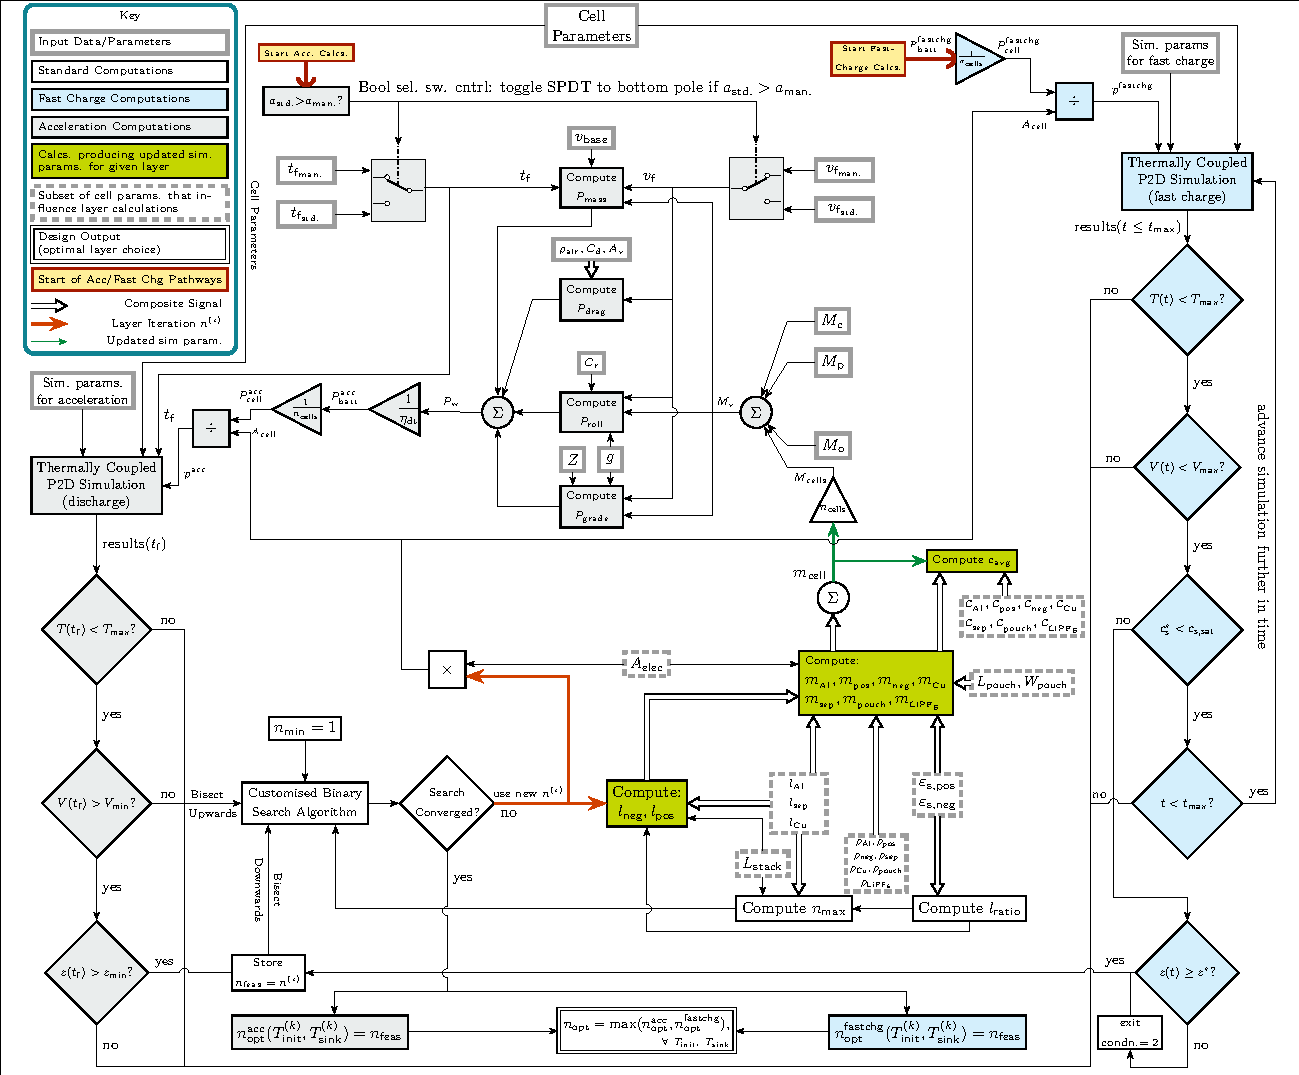
\includegraphics[angle=90, width=\textwidth]{fig_master_flow_diagram}
        \captionsetup{labelsep=note}
        \caption
        [%
        Flow diagram depicting an overview of the proposed layer optimisation methodology
        for Li-ion pouch cells.
        ]%
        {%
            Flow diagram depicting an overview of the proposed layer optimisation methodology
            for Li-ion pouch cells.
        }%
        \label{fig:fig_strategy_schematic}
        \mpfootnotes[1]
        % \vspace*{1.125cm}
        \vspace*{0.7225cm}
        \footnote{This figure was created by \mbox{Krishnakumar Gopalakrishnan} who
            asserts copyright, with intellectual contributions from and the right to
        use asserted by \mbox{Ian Campbell}.}
    \end{minipage}
\end{figure}

As explained in the legend key of \cref{fig:fig_strategy_schematic}, blocks with
a light  grey border  represent input  data/parameters for  computations. Blocks
with a standard black border  represent computations common to both acceleration
and fast  charging pathways. The design  output is given by  the double-bordered
block at the bottom centre  of \cref{fig:fig_strategy_schematic}. Other types of
blocks  and arrows  are  appropriately listed  in  the legend  key.  To aid  the
understanding of the  layer optimisation framework, the reader  is encouraged to
correlate  the narrative  in this  section  with the  blocks and  arrows in  the
schematic.



\subsection{Acceleration pathway}

The computations for acceleration-based layer  optimisation begins at the anchor
block labelled `Start Acc.\ Calcs.'.

\subsubsection*{Determination of acceleration rate, final speed and acceleration time}

The  first   step  is  the  determination   of  the  rate  of   acceleration  to
be  used  for  the  computing   the  power  requirements  for  accelerating  the
\gls{xeV}  from  standstill.  For  the  sake of  claiming  green  subsidies  and
other  regulatory reasons,  vehicular  standards for  electrified transport  are
codified by  various regulatory agencies  and standardisation bodies  (\eg{} the
SAE~J1772 standard~\cite{Sae2010}).  These typically specify a  minimum required
acceleration  rate for  the vehicle  under consideration  to be  certified as  a
road-faring electric vehicle. Manufacturers have their own specifications, which
typically exceed the minimum standards. However, for certain classes of electric
vehicles such  as golf  carts, the  manufacturer-specified standards  might fall
below that of a  roadworthy electric vehicle. In this case,  this thesis errs on
the side of conservative design by choosing the higher of the two values.

The   acceleration   rate   is   taken   to   be   the   simple   ratio   of   a
pre-determined  final  speed~$v_\text{f}$  to  the time  taken  to  attain  that
speed  from  standstill~$t_\text{f}$.  The  manufacturer-specified  acceleration
rate~$a_\text{man.}$ is compared against the minimum acceleration rate specified
by vehicular  standards~$a_\text{std.}$. The two \gls{spdt}  switches assign the
final speed~$v_\text{f}$  and acceleration time~$t_\text{f}$ to  the values from
the  appropriate source  depending on  which of  the two  acceleration rates  is
higher.

\subsubsection*{Computation of acceleration power at the wheels}

The  next  step  is  to  calculate   the  acceleration  power  required  at  the
driving wheels~$P_\text{w}$.  Using the  governing equations from  basic vehicle
dynamics~\cite{Maksimovic2012}, the power at the wheels is given by
\cref{eq:wheelpower}.
\begin{subequations}\label{eq:wheelpower}
    \begin{align}
        P_\text{w}     & = P_\text{mass} + P_\text{drag} + P_\text{roll} + P_\text{grade} \tag{\ref*{eq:wheelpower}}                  \\
        P_\text{mass}  & = \frac{1}{2} \frac{M_\text{v}(n)}{t_\text{a}} \left(v_\text{b}^2 + v_\text{f}^2\right) \label{eq:masspower} \\
        P_\text{drag}  & = \frac{1}{2} \left(\rho_\text{air} C_\text{d} A_\text{v}v_\text{f}^3\right) \label{eq:dragpower}            \\
        P_\text{roll}  & = C_\text{r} M_\text{v}(n) g v_\text{f} \label{eq:rollpower}                                                 \\
        P_\text{grade} & = M_\text{v}(n) Z g v_\text{f} \label{eq:gradepower}
    \end{align}
\end{subequations}

The  individual  components  contributing   to  the  summation  for  wheel-power
computation   presented   in    \cref{eq:wheelpower}   is   briefly   explained.
$P_\text{mass}$~represents  the  power  required  to  accelerate  the  vehicle's
mass.  $P_\text{drag}$~denotes the  power  required to  overcome air  resistance
while $P_\text{roll}$~represents  that required to overcome  rolling resistance.
Finally,  $P_\text{grade}$~represents the  power  required to  negotiate a  road
gradient.  Except  for  $M_\text{v}(n)$  which  is  described  next,  all  terms
in  the  \gls{rhs}  of  \crefrange{eq:masspower}{eq:gradepower}  are  constants.
Each  of  these  terms   is  explained  in  tables~\ref{tbl:CommonVehicleParams}
and~\ref{tbl:UniqueVehicleParams}  along with  their  numerical  values used  in
simulation.

\subsubsection*{Computation of layer-dependent vehicle mass}

Changing  the layer  count used  in  each cell  changes  the mass  of the  cell.
This  in-turn  affects the  mass  of  the  pack,  which further  influences  the
overall  vehicle  mass.  Thus,  for precise  computation  of~$P_\text{mass}$  in
\cref{eq:masspower},  $M_\text{v}(n)$  is  the  vehicle's  mass  computed  as  a
function of number of layers~$n$.

In  the  schematic  of~\cref{fig:fig_strategy_schematic},  this  layer-dependent
calculation of  mass of all cells  in the pack~$M_\text{cells}$ is  shown by the
product of  the signal  labelled $m_\text{cell}$ and  the triangular  gain block
representing the overall number of cells in the pack~$n_\text{cells}$.
\begin{equation}\label{eq:massofallcells}
    M_\text{cells} = n \times m_\text{cell}
\end{equation}

The   mass    of   the   vehicle    is   given    by   the   sum    of   chassis
mass~$M_\text{c}$,  vehicle  payload  $M_\text{p}$, pack  overhead  $M_\text{o}$
and  the  layer-dependent  mass  of  all  cells  in  the  pack  $M_\text{cells}$
shown   in   \cref{eq:massofallcells}.   The    computation   of   mass   of   a
single   cell    $m_\text{cell}$   is    detailed   in   the    section   titled
\hyperlink{href:layerdependentcellmass}{`Computation  of   layer-dependent  cell
mass'}.

\subsubsection*{Computation of acceleration power density per layer}

Since the \gls{p2d} equations of the \gls{dfn} model are based upon a normalised
unit area and is  applicable only to each electrochemical layer,  the goal is to
compute the  power density experienced  by each layer. This  is arrived at  by a
sequence of simple scaling steps.

Firstly, the  power demanded at  the pack terminals  is computed by  scaling the
power  at the  wheels  by the  efficiency  of the  drivetrain.  As explained  in
\cref{subsec:layeroptassumptions},  the  drivetrain  consists  of  a  number  of
components, the efficiencies of which depend on the operating point (such as the
speed and torque  of the electric motor, current drawn  by the power electronics
etc.). Following the  assumptions detailed in \cref{subsec:layeroptassumptions},
a  single lumped  efficiency~$\eta_\text{dt}$ can  be used  for the  powertrain.
The  pack  power  demand  $P^\text{acc}_\text{batt}$  is  then  divided  by  the
number  of cells  in the  pack $n_\text{cells}$  to obtain  the power  demand at
the  input of  the cell's  terminals~$p^\text{acc}_\text{cell}$. For  each layer
choice~$n$, the electrochemically active surface area is computed using by using
\cref{eq:overallarea},  wherein the  electrochemically active  surface area  per
layer~$A_\text{elec}$ listed in \cref{tbl:lcoSimParamslayeropt} is held constant
throughout.  Finally, the  acceleration power  density per  layer~$p^\text{acc}$
is  computed  by  dividing  $p^\text{acc}_\text{cell}$ by  the  overall  surface
area~$A_\text{cell}$.

\subsubsection*{Thermally-coupled \glsfmtshort{p2d} simulation and exit
conditions}\label{sec:accexitconditions}

For the  present layer choice~$n$,  a thermally-coupled \gls{p2d}  simulation is
performed for a duration of $t_\text{f}$  seconds with the applied power density
$p^\text{acc}_\text{cell}$ corresponding to the present layer choice as input.
When the simulation terminates, the cell's condition is compared against three
criteria ----
\begin{enumerate}
    \item the maximum possible values of cell temperature~$T_\text{max}$,
    \item the minimum allowed terminal voltage~$V_\text{min}$ and
    \item the lowest allowed cell \gls{soc}~$z_ztext{min}$.
\end{enumerate}
This helps to determine whether the cell constructed from the present layer
choice is able to successfully satisfy the acceleration power demands. These
comparison operations are represented by decision blocks placed in the leftmost
region of the schematic in~\cref{fig:fig_strategy_schematic}.

If  any one  of the  three  aforementioned exit  checks fails,  then that  layer
configuration is deemed  to be not feasible and the  entire workflow is repeated
by trialling a new layer choice.  A sophisticated search algorithm, described in
\cref{sec:searchalgo}, is employed  to minimise the number  of iterations needed
until a successful layer choice is obtained.

\subsubsection*{Search algorithm}\label{sec:searchalgo}

A  customised binary  search algorithm  is  employed in  the layer  optimisation
framework. The  binary search  algorithm is  a computationally  efficient search
algorithm requiring  a worst-case operational  count of $\mathcal{O}(k  \log k)$
where $k$ is  the overall number of  candidates to be searched.  The same search
strategy may be  used for both acceleration and fast  charging pathways although
the method is briefly described here in the context of the acceleration runs.

If   the  three   conditions  described   in  \cref{sec:accexitconditions}   are
successfully  met,  the output  of  the  binary search  algorithm  is  set to  a
logical~1.  If any  of these  conditions  fail, then  the output  is assigned  a
logical~0. Thus, the  search vector in this customised  search strategy consists
of  only two  possibilities,~0 and~1.  For very  low layer  counts, the  applied
power  densities  are very  high.  Therefore,  one  of  the exit  conditions  in
\cref{sec:accexitconditions} is likely to fail.  For very high layer counts, the
power  densities  are  very  low,  implying  that  acceleration  runs  shall  be
successful.  There exists  a critical  transition point  \viz{} the  first layer
count for  which the exit  condition toggles from~0  to~1. Through a  process of
systematically bisecting the layer search space, the optimal layer value can be
arrived at. An alternative to using the

\subsubsection*{\hypertarget{href:layerdependentcellmass}{Computation of layer-dependent cell mass}}\label{sec:massofonecell}

\subsection{Electrode thickness ratio for capacity balancing}\label{sec:electroderatio}

A key  idea of the layer  optimisation scheme is that  for computing the
physical  lengths  of electrode  as  a  function  of number  of  layers,
the  ratios  of  their thicknesses~$l_\text{ratio}$  is  held  constant.
This  coefficient is  germane to  the concept  of capacity  balancing of
electrodes  to equalise  their loading and is computed as follows.

Equating  the active material volume of both electrodes,
\begin{equation}
    A_\text{elec,pos}l_\text{pos}  \varepsilon_\text{s,pos} = A_\text{elec,neg}l_\text{neg}  \varepsilon_\text{s,neg} \label{eq:electrodeCapacity}\\
\end{equation}

Neglecting  overhangs   of  the  negative  electrode   (typically  below
$\SI{2}{\milli\meter}$ to  avoid plating  at the edges),  both electrode
materials have the same cross-sectional area~$A_\text{elec}$. Therefore,
\cref{eq:electrodeCapacity} reduces to
\begin{align}
    \cancel{A_\text{elec}}l_\text{pos}  \varepsilon_\text{s,pos} & = \cancel{A_\text{elec}}l_\text{neg}  \varepsilon_\text{s,neg}  \\
    l_\text{pos}  \varepsilon_\text{s,pos}                       & = l_\text{neg}  \varepsilon_\text{s,neg}\label{eq:electrodeCapequalarea}
\end{align}

For the reference cell under consideration, the length and breadth of the cell's
pouch is  obtained from the \gls{bev}  manufacturer~\cite{GMBoltBatteryDims} and
are listed in \cref{tbl:lcoSimParamslayeropt}.

% % double-check if electrode area or overall area or what ? And uncomment later
% on


% As  a  first-order  approximation  the
% product of  these dimensions can  be assumed  to be the  active material
% cross-sectional  area   (although  in  practice,  the   planar  area  of
% the  stack  needs to  be  slightly  smaller  to be  accommodated  inside
% the  pouch).  Finally,  in  line   with  the  assumptions  discussed  in
% \cref{subsec:layeroptassumptions},  similar  to  the pouch  height,  the
% cross-sectional geometry (length  and breadth) of the cell  is also held
% constant throughout the layer optimisation process.

Owing to the reasons  outlined in \cref{subsec:layeroptassumptions}, the
volume fractions of the electrode  materials are assumed to be constant,
which  implies  that their  ratio  is  also  a constant.  The  electrode
thickness ratio~$l_\text{ratio}$ is obtained as
\begin{alignat}{2}
    l_\text{ratio} & = \frac{l_\text{neg}}{l_\text{pos}}                                                                                  &  & \qquad\text{(by definition)}                                          \\
    {}             & = \frac{\varepsilon_\text{s,pos}}{\varepsilon_\text{s,neg}}                                                          &  & \qquad\text{(rearranging \cref{eq:electrodeCapequalarea})}           \\
    {}             & = \frac{1-\varepsilon_\text{pos} - \varepsilon_\text{fi,pos}}{1-\varepsilon_\text{neg} - \varepsilon_\text{fi,neg}}  &  & \qquad\text{(by definition)}                                          \\
    {}             & = \frac{1- 0.385 - 0.025}{1 - 0.485 - 0.033}                                                                         &  & \qquad\text{(substituting values from \cref{tbl:lcoSimParamsSPMp2d})} \\
    l_\text{ratio} & = 1.22\label{eq:electrodeThicknessRatio}
\end{alignat}

% Do not forget to quote the value of cs_sat from layer opt paper table and show
% calculation inline. Might even go into the code

\subsection{Power inputs considered}

P2D model  equations are developed  for bi-directional input power.  xEV battery
pack has  constant power input,  if the  installed power capability  of charging
stations  is  fully  utilised.  Equation  (1)  describes  vehicle  dynamics  for
acceleration  and  power  demand.  For  fast  charging,  the  power  electronics
components of all grid chargers possess  a peak power delivery rating.
